	\subsubsection{Modal de Gerenciamento de Atribuições}

\begin{center}
	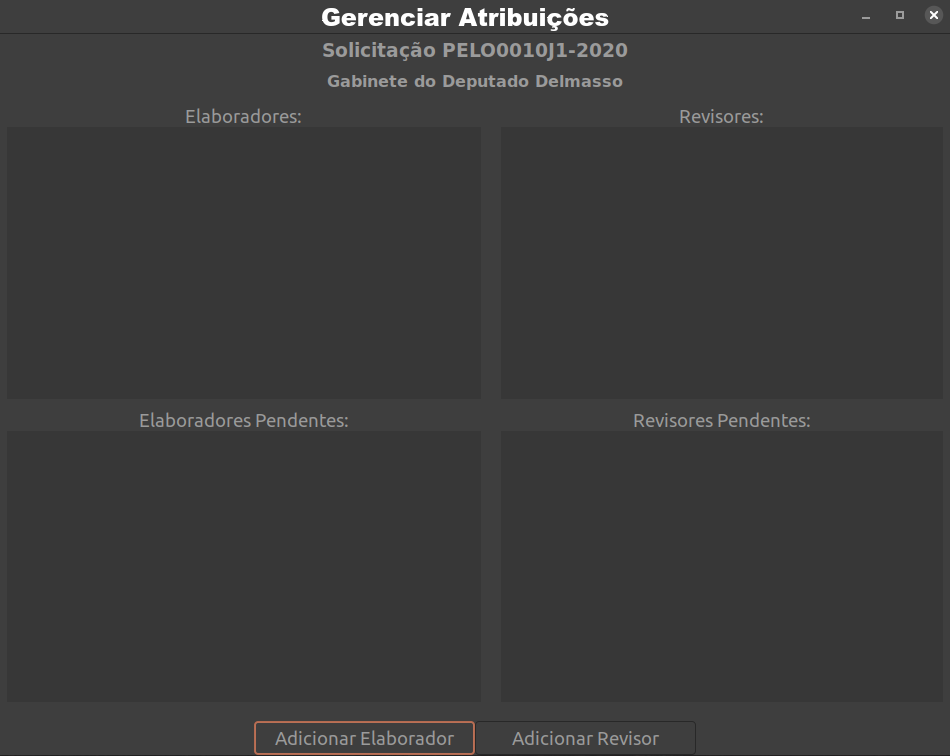
\includegraphics[width=0.9\textwidth]{fig/ger-sol-unid/ger-atrib.png}
\end{center}

A figura acima mostra um protótipo do que poderia ser o \textbf{modal de ``Gerenciamento de Atribuições''} para uma determinada solicitação. Trata-se de uma janela com 4 listas para exibir a situação das atribuições de consultores para uma dada solicitação:

\begin{itemize}
	\item  \textbf{Elaboradores}: Na lista esquerda superior são exibidos os nomes dos consultores atuando na solicitação como \textbf{elaboradores}. Seja qual for a modalidade de atribuição utilizada nesta atribuição, os consultores dessa lista já estão atuando na solicitação. 
	
	\item \textbf{Elaboradores Pendentes}: Na lista esquerda inferior são exibidos os nomes dos consultores que foram atribuídos à solicitação na qualidade de \textbf{elaborador}, mas que ainda não aceitaram a atribuição. Neste caso eles foram adicionados pela modalidade ``empurra'' e, portanto, precisam aceitar a atribuição. Enquanto não aceitarem, seus nomes aparecem na lista de elaboradores pendentes. Depois que aceitarem, quando algum supervisor acessar esse modal novamente, seu nome já estará na lista de cima.
	
	\item \textbf{Revisores}: De forma semelhante, na lista direita superior são exibidos os nomes dos consultores atuando na solicitação como \textbf{revisores}.  
	
	\item \textbf{Revisores Pendentes}: E na lista direita inferior estão os nomes dos consultores atribuídos como revisores mas que ainda não aceitaram a atribuição.
\end{itemize}

O modal também teria botões com funções. Na figura são exibidos apenas botões para adicionar consultores como elaboradores e revisores, mas ao todo seriam interessante termos pelo menos os seguintes botões:

\begin{itemize}
	\item \textbf{Adicionar Elaborador}: Adiciona um consultor na qualidade de elaborador para a solicitação colocando ele na lista de elaboradores pendentes e modifica os estados da ``Área de Trabalho do CL'' do consultor adicionado como elaborador para que ele aceite essa atribuição notificando-o deste evento. 
	
	\item \textbf{Adicionar Revisor}: Adiciona um consultor na qualidade de revisor para a solicitação colocando ele na lista de revisores pendentes e modifica os estados da ``Área de Trabalho do CL'' do consultor adicionado como revisor para que ele aceite essa atribuição notificando-o deste evento.
	
	\item \textbf{Remover}: 
	
	\begin{itemize}
		\item Se o consultor selecionado para remoção estiver na lista de elaboradores então manda notificação e aguarda aceite para ser removido. 
		\item Se o consultor selecionado para remoção estiver na lista de elaboradores pendentes então manda notificação e realiza a remoção modificando estados da ``Área de Trabalho do CL''. 
		\item Idem caso o consultor selecionado para remoção estiver na lista de revisores. 
		\item Idem caso o consultor selecionado para remoção estiver na lista de revisores pendentes. 
	\end{itemize}
\end{itemize}


\subsubsection{Modal de Gerenciamento de Inscrições}

O modal de gerenciamento de inscrições, de acesso exclusivo de supervisores, deve listar as solicitações que possuem consultores que se escreveram para atuar como elaboradores ou revisores, mas cujo consentimento do supervisor ainda não foi dado. Esse modal só estará disponível caso alguma das variáveis de configuração que controla a dispensa de consentimento não esteja habilitada.

Dessa forma, se uma determinada unidade deseja que o supervisor gerencie pedidos de auto-atribuição em solicitações aceitando ou rejeitando esses pedidos, aqui será o lugar onde os supervisores poderão realizar esses eventos.

\begin{nota}{Protótipo do modal de gerenciamento de inscrições}
	O protótipo, que ainda precisa ser desenhado, precisa listar somente solicitações da unidade com pedidos de inscrições não aprovadas. Precisa dizer, para cada solicitação, qual consultor se inscreveu e para que qualidade: elaborador ou revisor.
	
	Ainda devem haver botões para que os supervisores aceitem ou rejeitem os pedidos de inscrição. Ao rejeitar um pedido, o supervisor deve poder escrever uma motivação que será transformada em artefato observação da solicitação.
\end{nota}


%%%%%%%%%


\subsection{Tabela de Solicitações a cargo do CL} 	

Ela basicamente lista as solicitações que estão a cargo do \CL atuar e deve conter os seguintes grupos de colunas:

\begin{itemize}
	\item \textbf{Propriedades da Solicitação}: São colunas que devem exibir algumas propriedades da solicitação. Aqui no mínimo: o \textbf{código identificador} e a \textbf{unidade solicitante}.
	
	
	\item \textbf{Controle do CL}: Grupo de colunas parecidos com os definidos no módulo das unidades, mas com colunas para controle das solicitações pelo \CL:
	
	\begin{itemize}
		\item \textbf{Urgente}: Exibe propriedade ``urgente'' conforme definido pela ASSEL. Não permite que o CL altere o estado. 
		
		\item \textbf{Prioridade}: Exibe propriedade ``prioridade'' conforme definido pela Unidade. Não permite que o CL altere o estado.
		
		\item \textbf{Tempo Atribuído}: Campo auto-calculado pelo sistema que exibe a quantidade de tempo dado pela diferença entre o instante de tempo atual e o instante em que a solicitação foi atribuído ao CL para atuar como elaborador ou revisor.
	\end{itemize}
	
	\item \textbf{Estado da Solicitação}: Colunas parecidas com aquelas da unidade:
	\begin{itemize}
		\item \textbf{Estado para o CL}: Exibe o estado para o \CL em que uma solicitação encontra-se. Veja que aqui os estados são diferentes pois contempla os estados adicionais transitórios ``Aceitar Elaboração'', ``Aceitar Revisão'', ``Aguardando consentimento para elaboração'' e ``Aguardando consentimento para revisão'' além dos estados ``Em Elaboração'' e ``Solicitação Concluída''.
		
		\item \textbf{Elaborador(es)}: Lista os \CLs atribuídos à solicitação na qualidade de elaboradores.
		
		\item \textbf{Revisor(es)}: Lista os \CLs atribuídos à solicitação na qualidade de revisores.
	\end{itemize}
\end{itemize}


\begin{nota}{Definição de Colunas Exibidas}
	Da mesma forma, a definição final de quais colunas serão exibidas na tabela ainda não foi estabelecida pois há uma restrição de espaço e, portanto, depende de mais reuniões com os líderes de negócios.
\end{nota}
